\section{双拐点暴胀模型}
拐点暴胀通常指这样的暴胀模型,存在场值$\phi=\phi_0$(拐点)使得势能在该处的二阶导数为零
\begin{equation}
    V^{\dprime}(\phi_0) = 0
\end{equation}

势能的一般形式为

\begin{equation}
    \label{eq:inf_potential}
    V (\phi)=V_0+a (\phi-\phi_0)+\frac{c}{6}{\left(\phi-\phi_0\right)}^3\\
\end{equation}
\begin{equation}
    V_0\equiv V (\phi_0),\ a\equiv V' (\phi_0),\ c\equiv V^{\tprime} (\phi_0) 
\end{equation}

高阶项 $(n \geq 4)$ 被截断。相应的慢滚参数为
\begin{equation}
    \label{eq:psrp}
    \epsilon = \frac{M_p}{2}\left(\frac{V'}{V}^2\right),\ \eta=M^2_p
    \left(\frac{V^{\dprime}}{V}\right),\ \xi^2=M^4_p\left(\frac{V'V^{\tprime}}{V^2}\right)
\end{equation}

接下来通过WMAP、Planck等实验观测到的标量扰动大小$\mathcal{P}_R$和标量谱指标$n_s$来确定系数a和c。
令暴胀结束时的场值为$\phi_e$,那时有$\epsilon\sim
1$。则对应$\phi\sim\phi_e$的e-folding数为
\begin{align}
    \label{eq:e-folding}
    \mathcal{N} &= \frac{V_0}{M^2_p}\sqrt{\frac{2}{ac}}\lbrack
    F_0(\phi_e)-F_0(\phi)\rbrack \\
    F_0(z) &= \cot^{-1}\left(\sqrt{\frac{c}{2a}}(z-\phi_0)\right)
\end{align}

如果将慢滚参数在极值处的平方根定义为 $X$, $\mathcal{N}$ 中涉及 $\phi$
的部分定义为 $Y$,那么可以将各慢滚参数及可观测量用统一用$X,Y$进行描述。

\begin{align}
    \epsilon &=
    \frac{2V_0^2}{c^2M_p^6\mathcal{N}^4} {\left(\frac{Y}{X} \right)}^4 \\
    \eta &=
    -\frac{2}{\mathcal{N}}\frac{Y}{S}\left(\sqrt{1-X}\cos Y-\sqrt{X}\sin
    Y\right)\\
    \xi^2 &= \frac{2}{\mathcal{N}^2}{\left(\frac{Y}{X}\right)}^2
\end{align}

在暴胀期间,$\epsilon \ll 1$,导致$X=S\sqrt{\epsilon}\leq\sqrt{\epsilon}\ll
1$,故而有$S\approx \sin Y$。相应的功率谱,标量谱指标及其跑动为
\begin{align}
    \mathcal{P}^{1/2}&\equiv\frac{1}{\sqrt{24\pi^2}}\frac{V_0^{1/2}}{\epsilon^{1/2}M_p^2}
    \approx\frac{V_0^{1/2}}{2\sqrt{6}\pi M_p^2 X}\sin^2Y\\
    n_s&\equiv1+2\eta-6\epsilon\approx1-\frac{4}{\mathcal{N}}Y\cot Y\\
\end{align}
\section{超引力}

仍然考虑带有平移对称性的K\"ahler势\citep{ketov2016susy}
\begin{align}
    K=ic(\Phi-\bar\Phi)-\frac{1}{2}{(\Phi-\bar\Phi)}^2-\frac{\zeta}{4}{(\Phi-\bar\Phi)}^4,
\end{align}
其中$c$和$\zeta$为实参数。暴胀场取为手征超场$\Phi=(\phi+i\chi)/\sqrt{2}$的实部分量$\phi$。只要四次方项$\frac{\zeta}{4}{(\Phi-\bar\Phi)}^4$中的$\zeta$取得足够大,则暴胀场$\phi$在暴胀期间,场$\chi$的期望为$\langle\chi\rangle\approx0$。

参考了racetrack模型\citep{krasnikov1987supersymmetry,escoda2003saltatory,blanco2005racetrack}和其他模型\citep{ketov2016susy},我们选取如下形式的超势
\begin{align}
    W=a_0(1+a_1e^{-b_1\Phi}+a_2e^{-b_2\Phi}+a_3e^{-b_3\Phi}).
\end{align}

如果我们在宇宙学常数为零的真空中恢复来真空的超对称性(关于真空中的超对称破缺问题的讨论请参考文献\citep{gao2015inflection}),则F-term和势能V在$\Phi=0$处应当都为零,即$D_{\Phi}W=0$,$V=0$,这要求超势W满足约束条件
\begin{align}\label{eq:sp_constrain}
    W=\partial_{\Phi}W=0.
\end{align}
求解约束条件 (\ref{eq:sp_constrain}) 可以消去参数$a_1$和$a_2$
\begin{align}
    a_1\rightarrow \frac{b_2+a_3b_2-a_3b_3}{b_1-b_2},\qquad 
    a_2\rightarrow \frac{-b_1-a_3b_1+a_3b_3}{b_1-b_2}.
\end{align}
将K\"ahler势和超势代入到公式
\begin{align}
    V=e^{K/M^2_P}\lbrack
    D_{\Phi_i}W{(K^{-1})}^{ij^{\star}}D_{\Phi^{\star}_j}W^{\star}-3M^{-2}_P|W|^2\rbrack,
\end{align}
中,可以得到标量势能$V(\phi)$。其中,
\begin{align}
    D_{\Phi}W=\partial_{\Phi}W+M^{-2}_P{(\partial_{\Phi}K)}W,
\end{align}
以及K\"ahler度规的逆,
\begin{align}
    K^{ij\star} = \frac{\partial^2K}{\partial\Phi_i\partial\Phi^{\star}_j}.
\end{align}

当在参数空间中选取某组参数如
\begin{align}\label{eq:parameters}
    a_0 = 4.35\times 10^{-6},
    a_3 = 7\times 10^{-8},
    b_1 = 3.05,
    b_2 = 6.3868164,
    b_3 = -4.4,
    c = 2.8.
\end{align}
时,标量势能$V(\phi)$有两个近反射点,如图\ref{fig:potential}中所示。场取较大值处的拐点给出与当前CMB数据相一致的标量谱指标和张标比,较小值处的拐点可以使标量扰动的功率谱产生一个尖峰从而生成原初黑洞。
\begin{figure}[!htbp]
    \centering
    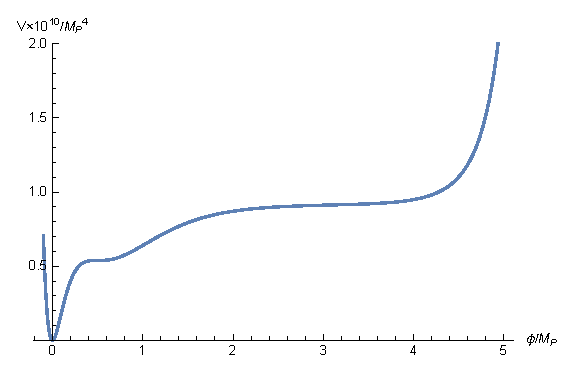
\includegraphics{Img/potential.eps}
    \caption{双拐点标量势能$V(\phi)$}\label{fig:potential}
\end{figure}

在FRW背景以及单场慢滚框架下,基于势能的慢滚参数$\epsilon_V$和$\eta_V$为
\begin{align}
    \epsilon_V &= \frac{M^2_P}{2}{\left(\frac{V\prime}{V}\right)}^2, \\
    \eta_V &= M^2_P {\left(\frac{V^{\prime\prime}}{V}\right)}.
\end{align}

由于在拐点附近势能变得极端平坦,因此慢滚近似不再适用\citep{dimopoulos2017ultra,germani2017primordial},代之以极端慢滚暴胀。此时为了更精确地求解暴胀过程,势能慢滚参数需要替换为哈勃慢滚参数\citep{schwarz2001higher,leach2002cosmological,schwarz2004primordial},
\begin{align}
    \epsilon_H &= -\frac{\dot{H}}{H^2}, \\
    \eta_H &= -\frac{\ddot{H}}{2H\dot{H}}=\epsilon_H-\frac{1}{2}\frac{d \ln\epsilon_H}{dN_e}, \\
    \xi_H &=
    \frac{\dddot{H}}{2H^2\dot{H}}-2\eta^2_H=\epsilon_H\eta_H-\frac{d\eta_H}{dN_e},
\end{align}

点$\dot{}$表示对宇宙时间$t$的导数,$N_e(t)$表示从视界穿过$k_{\star}$到暴胀结束期间的e-folding数,通常在取值在范围$50\sim60$之间。

标量谱指标及其跑动和张标比的领头阶可以用$\epsilon_H,\eta_H,\xi_H$来表示
\begin{align}
    n_s &= 1- 4\epsilon_H+2\eta_H, \\
    \alpha &= \frac{dn_s}{d\ln k}=10\epsilon_H\eta_H-8\epsilon_H^2-2\xi_H, \\
    r &= 16\epsilon_H.
\end{align}

在参数集 (\ref{eq:parameters}),相应的数值结果为
\begin{align}
    n_s = 0.9635,\qquad \alpha=-0.00369,\qquad r=0.00276,
\end{align}

当$k_{\star}=0.05Mpc^{-1}$时,在$68\%$的置信水平上与Planck
2018给出的对CMB的限制结果相一致\citep{akrami2018planck}
\begin{align}
    n_s = 0.9640\pm 0.0043,\qquad 
    \alpha = -0.0071\pm 0.0068,\qquad
    r < 0.079.
\end{align}

由于在拐点附近用近似表达式$\mathcal{P_R}\approx\frac{1}{8\pi^2M^2_P}\frac{H^2}{\epsilon_H}$计算得到的标量扰动会低于真实值\citep{gao2018primordial}。因此必须在模空间中数值求解MS方程,
\begin{align}\label{eq:ms}
    \frac{d^2u_k}{d\eta^2}+\left(k^2-\frac{1}{z}\frac{d^2z}{d\eta^2}\right)u_k=0,
\end{align}
其中$\eta$为共形时间,$z\equiv\frac{a}{\mathcal{H}}\frac{d\phi}{d\eta}$。初值条件取为Bunch-Davies真空\citep{bunch1978quantum}
\begin{align}
    u_k\rightarrow\frac{e^{-ik\eta}}{\sqrt{2k}},\quad\text{as}\quad
    \frac{k}{aH}\rightarrow\infty.
\end{align}

出于数值求解的方便,我们将共形时间$\eta$替换为$N_e$,把MS方程重写为\citep{ballesteros2018primordial}
\begin{align}
    \frac{d^2u_k}{dN^2_e}+\left(1-\epsilon_H\right)\frac{du_k}{dN_2}+
    \lbrack\frac{k^2}{\mathcal{H}^2}+\left(1+\epsilon_H-\eta_H\right)\left(\eta_H-2\right)-\frac{d\left(\epsilon_H-\eta_H\right)}{dN_e}=0,
\end{align}
原初功率谱由下式给出
\begin{align}
    \mathcal{P_R}=\frac{k^3}{2\pi^2}\lvert\frac{u_k}{z}\rvert^2_{k\ll
    \mathcal{H}}
\end{align}

图\ref{fig:pert}为MS方程\ref{eq:ms}基于参数集\ref{eq:parameters}的数值结果。从图中可以发现功率谱在小尺度有一个高峰,在CMB的尺度上大约增长了7个数量级。这样大的一个密度扰动使得原初黑洞能够通过引力塌缩形成。

\begin{figure}[!htbp]
    \centering
    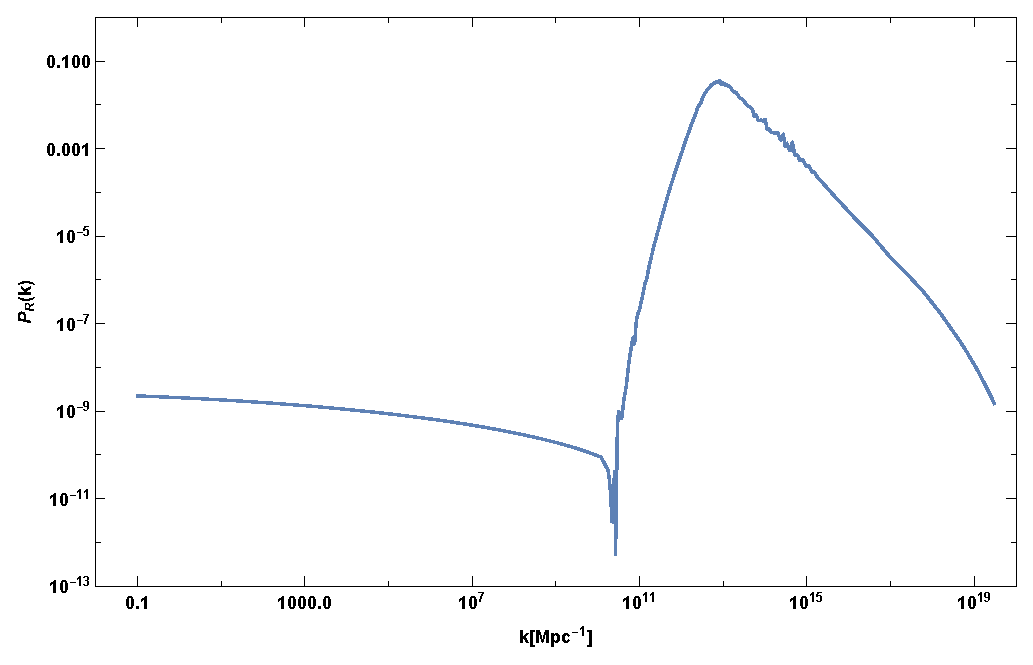
\includegraphics[width=4in]{Img/pert.eps}
    \caption{双拐点暴胀模型预测的标量扰动的原初功率谱$\mathcal{P_R}$}\label{fig:pert}
\end{figure}
